% ============================================================
%  Capítulo 4 — Dataset
% ============================================================
\chapter{DATASET}
\label{cap:dataset}

\section{Configuração do crawl}
\label{sec:crawl-config}

\subsection{Seleção de sites}
\label{sub:sitios}

Os sites-alvo são os 10.000 primeiros da lista Tranco \cite{lepochat2019}, uma
classificação de popularidade de domínios baseada em múltiplas listas de tráfego
agregadas semanalmente. A Tranco é preferida em relação à lista Alexa por ser
reprodutível (cada versão é identificada por data e pode ser consultada
retroativamente) e por filtrar domínios de infraestrutura e CDN que distorcem
classificações baseadas em DNS puro.

O mesmo conjunto de 10.000 URLs é visitado pelos dois crawlers:
Firefox/SpiderMonkey e Chromium/V8. Isso garante que cada site contribua com dois
registros de bytecodes, um por motor, para o mesmo conjunto de chamadas de
API, tornando o dataset intrinsecamente cross-engine.

\subsection{Parâmetros de visita}
\label{sub:params}

Cada site é visitado uma única vez por navegador, com os seguintes parâmetros:

\begin{table}[htb]
\centering
\caption{Parâmetros de visita por crawler}
\label{tab:params}
\begin{tabularx}{\linewidth}{lXX}
\toprule
\textbf{Parâmetro} & \textbf{Firefox} & \textbf{Chromium} \\
\midrule
Timeout de carregamento             & 15\,s & 15\,s \\
Watchdog por site                  & 60\,s & 60\,s \\
Comportamento pós-carregamento      & scroll em 5 posições + digitação & scroll em 5 posições + digitação \\
Espera extra após FP detectado      & 2\,s  & 2\,s \\
Reinício do navegador               & a cada 30 sites & a cada 10 sites \\
\bottomrule
\end{tabularx}
\fonte{Elaborada pelo autor.}
\end{table}

O comportamento de scroll e digitação simula interação humana, ativando
event listeners de sites que iniciam a coleta de fingerprint apenas
após interação do usuário. O reinício periódico do Firefox controla o tamanho do
arquivo de log do geckodriver, que seria processado integralmente ao final de cada
batch. O reinício do Chromium foi feito com maior frequência por conta do maior consumo de memória acumulada entre sessões.

\subsection{Idempotência e retomada}
\label{sub:idempotencia}

Ambos os crawlers são idempotentes: registram URLs concluídas em arquivos
de progresso e retomam a partir da última URL pendente em caso de
reinicialização. Bytecodes são escritos
incrementalmente no arquivo JSONL de saída; chamadas de API são appended ao
arquivo correspondente após cada visita.

%, , , , , , , , , , , , , , , , , , , --
%, , , , , , , , , , , , , , , , , , , --
\section{Estatísticas do dataset}
\label{sec:stats}

\subsection{Dataset rotulado bruto}
\label{sub:stats-bruto}

Após o crawl completo dos 10.000 sites com ambos os navegadores e o
processamento pelo pós-processador, o dataset rotulado bruto apresenta
as seguintes características:

\begin{table}[htb]
\centering
\caption{Estatísticas do dataset rotulado bruto}
\label{tab:stats-bruto}
\begin{tabular}{ll}
\toprule
\textbf{Métrica} & \textbf{Valor} \\
\midrule
Funções totais                                            & 68.008.403 \\
Funções de fingerprinting (\texttt{is\_fp = True})        & 37.644 (0,055\%) \\
Funções não-FP                                            & 67.970.759 (99,945\%) \\
Tamanho do arquivo (Parquet, zstd)                        & 5,43~GB \\
\bottomrule
\end{tabular}

\fonte{Elaborada pelo autor.}
\end{table}

A proporção de 0,055\% de funções positivas é característica de crawls de
alta escala: a vasta maioria das funções JavaScript de uma página serve a
propósitos de interface, roteamento, gerenciamento de estado ou analytics, não
de fingerprinting. Esse nível extremo de desbalanceamento motiva a
estratégia de amostragem descrita na Seção~\ref{sec:amostragem}.

\subsection{Distribuição por categoria}
\label{sub:stats-cats}

Os rótulos multilabel não são mutuamente exclusivos: uma função pode ser
classificada em mais de uma categoria se suas chamadas de API satisfizerem os
critérios de múltiplas heurísticas. A Figura~\ref{fig:cats} apresenta a distribuição de funções por categoria relativo ao total de funções FP.

\begin{figure}[htb]
\centering
\caption{Distribuição de funções de fingerprinting por categoria (categorias não exclusivas).}
\label{fig:cats}
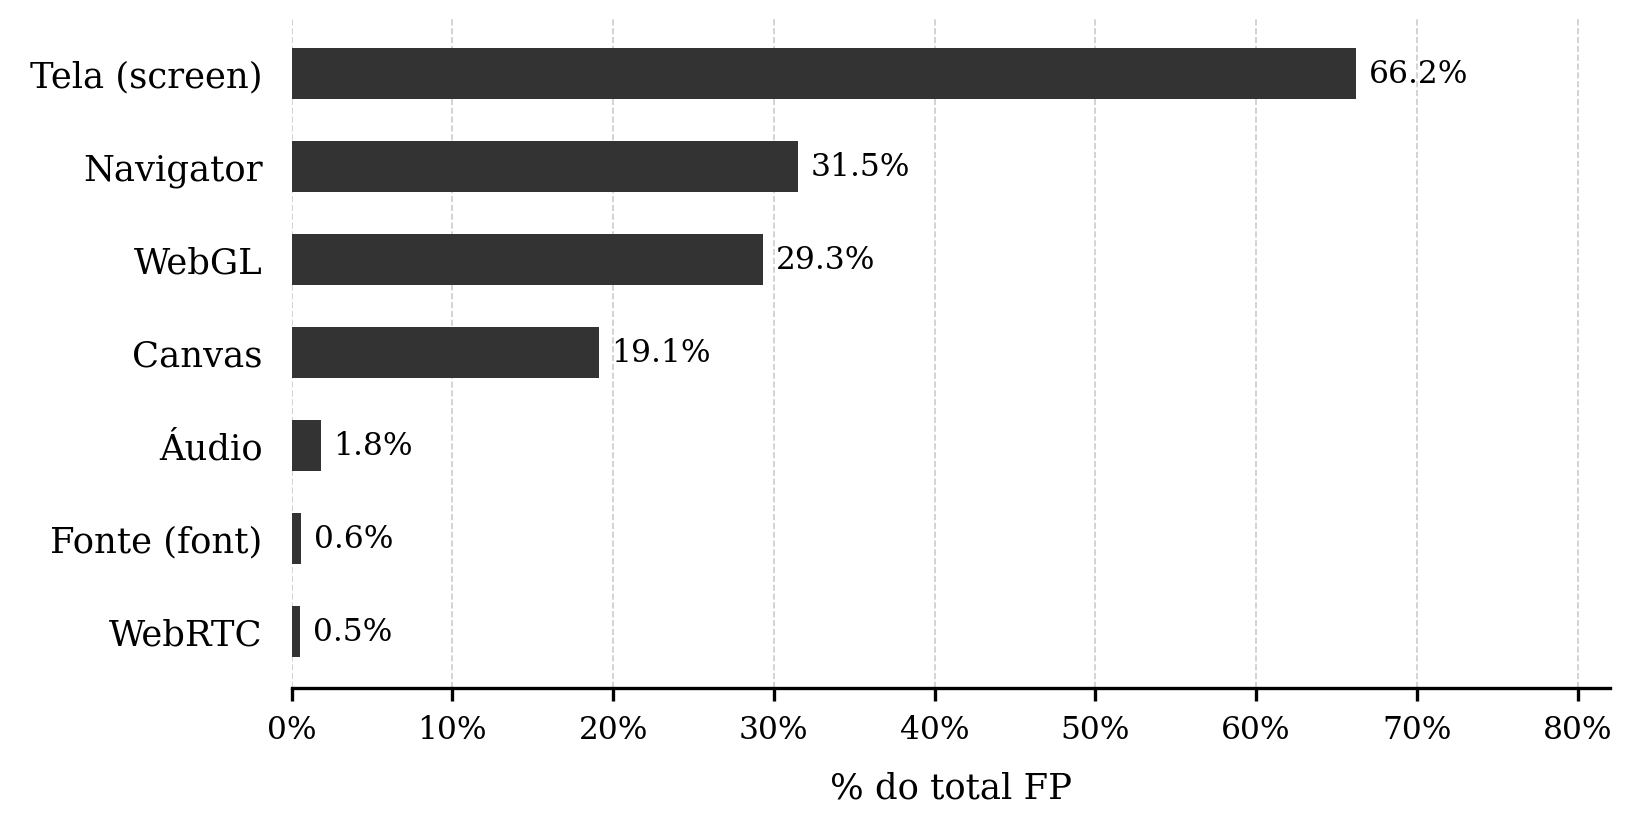
\includegraphics[width=0.82\linewidth]{fig_category_distribution}

\fonte{Elaborada pelo autor.}
\end{figure}

A Figura~\ref{fig:cats} ilustra graficamente essa distribuição. A assimetria é de
duas ordens de magnitude entre as categorias mais comuns (Tela, WebGL, Navigator)
e as mais raras (WebRTC, Fonte).
Categorias como Tela e Navigator são coletadas por praticamente qualquer biblioteca
de fingerprinting, enquanto WebRTC e Fonte aparecem apenas em
implementações mais agressivas, presentes em uma minoria dos sites do Top~10k.
Essa assimetria tem implicações diretas para o desempenho dos classificadores
multilabel, discutidas no Capítulo~\ref{cap:discussao}.

%, , , , , , , , , , , , , , , , , , , --
\section{Heurísticas ByteDefender para atribuição de rótulos multilabel}
\label{sec:heuristicas}

A atribuição de rótulos não é feita por inspeção manual nem por palavras-chave no
nome da função: as funções de fingerprinting têm nomes arbitrários,
especialmente em bundles minificados. Em vez disso, o pós-processador
implementa heurísticas baseadas no padrão de chamadas de API observado durante
a execução, seguindo a metodologia do ByteDefender \cite{nikkhahbahrami2025}.

Para cada função, o pós-processador agrega o conjunto de APIs chamadas, o
comprimento máximo do argumento de \texttt{fillText}, o número de chamadas a
\texttt{measureText}, o número de valores distintos do setter \texttt{font}, o
número de chamadas WebGL que expõem parâmetros de fabricante/renderizador e o
número de propriedades distintas de \texttt{navigator} acessadas. Com base
nesses agregados, cada heurística é avaliada como uma expressão booleana:

\textbf{Canvas.} Presença simultânea de \texttt{canvas.toDataURL} e
\texttt{canvas.fillText} com argumento de comprimento mínimo 10, combinada com
ausência de \texttt{canvas.save} e \texttt{canvas.restore}. Os critérios negativos
discriminam uso de canvas para renderização de interface, que frequentemente envolve
save/restore, do uso para extração de fingerprint, que não necessita dessas
operações.

\textbf{Áudio.} Presença simultânea de \texttt{audio.\allowbreak createOscillator},
\texttt{audio.\allowbreak createDynamicsCompressor}, \texttt{audio.\allowbreak startRendering},
\texttt{audio.\allowbreak connect} e pelo menos um entre \texttt{audio.\allowbreak getChannelData} e
\texttt{audio.\allowbreak copyFromChannel}. O padrão completo (oscilar, comprimir, renderizar offline, conectar e extrair o resultado) é a assinatura canônica da técnica de audio fingerprinting.

\textbf{WebRTC.} Presença de \texttt{webrtc.setLocalDescription} combinada com
\texttt{webrtc.createOffer} ou \texttt{webrtc.createDataChannel}. A negociação de
candidatos ICE, que expõe IPs locais, requer obrigatoriamente
\texttt{setLocalDescription}.

\textbf{Fonte.} Pelo menos 20 chamadas a \texttt{canvas.measureText} e mais de 20
valores distintos do setter \texttt{canvas.font}. A enumeração de fontes requer a
medição das dimensões de texto em dezenas de famílias tipográficas, daí os
limiares elevados.

\textbf{WebGL.} Pelo menos uma chamada a \texttt{webgl.getParameter} com um
parâmetro que exponha informações do fabricante ou do renderizador da GPU
(\texttt{RENDERER}, \texttt{VENDOR} ou constantes de extensão equivalentes).

\textbf{Tela.} Presença de \texttt{screen.colorDepth} ou
\texttt{screen.pixelDepth}, combinada com pelo menos uma entre
\texttt{screen.width}, \texttt{screen.height} e \texttt{screen.availWidth}. O
acesso isolado a dimensões de tela é comum em código responsivo legítimo; a
combinação com profundidade de cor é o indicador de fingerprinting.

\textbf{Navigator.} Pelo menos 3 propriedades distintas de \texttt{navigator}
acessadas dentre as monitoradas (\texttt{hardwareConcurrency}, \texttt{languages},
\texttt{platform}, \texttt{deviceMemory}, \texttt{maxTouchPoints}). O acesso a
uma ou duas propriedades pode ocorrer legitimamente; o acesso a três ou mais indica
coleta sistemática de perfil de hardware.

%, , , , , , , , , , , , , , , , , , , --
\section{Limpeza de ruído}
\label{sec:limpeza}

\subsection{Origem do ruído}
\label{sub:ruido-origem}

O dataset bruto contém tokens espúrios provenientes de dois mecanismos:

\textbf{Artefatos de cabeçalho de log.} A separação entre o prefixo de log e o
conteúdo JSON é feita por parsing de texto simples. Em casos de quebra de linha
inesperada, por exemplo, quando o sistema operacional interrompe uma escrita em
stderr, o prefixo \texttt{[V8Log]} ou \texttt{[SpiderMonkey Log]} pode
aparecer embutido dentro da string de bytecodes, gerando tokens como
\texttt{[SpiderMonkey}, \texttt{Log]} ou \texttt{Return[V8Log]}.

\textbf{Tokens truncados.} O geckodriver impõe um limite de comprimento por linha de
log do SpiderMonkey; o sistema operacional pode interromper escritas longas em stderr
para o V8. Funções com sequências de bytecodes muito longas têm as últimas sequências
truncadas, produzindo tokens parciais como \texttt{GetNam} (em vez de
\texttt{GetNamedProperty} no SpiderMonkey) ou \texttt{LdaConst} (em vez de
\texttt{LdaConstant} no V8) ou caracteres isolados como \texttt{S}, \texttt{C},
\texttt{L}.

\textbf{Normalização de formato.} O SpiderMonkey emite bytecodes com espaço após
a vírgula (\texttt{"A, B, C"}), enquanto o V8 não usa espaço (\texttt{"A,B,C"}).
O módulo de limpeza normaliza para o formato sem espaço.

\subsection{Regra de filtragem}
\label{sub:ruido-filtro}

Um token é considerado válido se e somente se corresponde à expressão regular:

\begin{lstlisting}[language={}]
^[A-Za-z][A-Za-z0-9_]{1,}$
\end{lstlisting}

A regra exige início com letra, comprimento mínimo de 2 caracteres e composição
exclusivamente alfanumérica com sublinhados. Tokens com colchetes, tokens de um
caractere e tokens truncados são descartados. Linhas cujos bytecodes ficam
completamente vazios após a filtragem são removidas do dataset.

\subsection{Resultado da limpeza}
\label{sub:ruido-resultado}

\begin{table}[htb]
\centering
\caption{Resultado da limpeza de ruído}
\label{tab:limpeza}
\begin{tabular}{ll}
\toprule
\textbf{Métrica} & \textbf{Valor} \\
\midrule
Linhas processadas                                            & 68.008.403 \\
Taxa de ruído de tokens                                       & 1,17\% \\
Arquivo de saída (Parquet limpo, zstd) & 5,10~GB \\
\bottomrule
\end{tabular}

\fonte{Elaborada pelo autor.}
\end{table}

A taxa de ruído de 1,17\% confirma que a maioria das sequências de bytecodes está
íntegra. Os tokens removidos concentram-se em um subconjunto pequeno de funções
com bytecodes muito longos (afetados pelo truncamento do geckodriver para o
SpiderMonkey ou por interrupções de escrita em stderr para o V8) e em funções
cujos scripts foram carregados durante reinicializações do navegador.

%, , , , , , , , , , , , , , , , , , , --
\section{Amostra de treinamento}
\label{sec:amostragem}

\subsection{Problema de escala e desbalanceamento}
\label{sub:escala}

O dataset limpo contém 68 milhões de funções. Carregar todas as sequências de
tokens em memória para treinamento de classificadores baseados em TF-IDF é
inviável: a matriz TF-IDF em formato denso (68M $\times$ 4.723~features de
bigrams, em \texttt{float32}) ocuparia aproximadamente 1,3~TB de RAM. Além disso, o
desbalanceamento de 1:1.806 (FP:não-FP) inviabiliza o treinamento direto sem
estratégia de amostragem.

\subsection{Sampler em dois passes}
\label{sub:sampler}

O amostrador opera em dois passes sobre o arquivo Parquet:

\textbf{Passo~1, estimativa de FP.} Um em cada 50 grupos de linhas (row
groups) do arquivo Parquet é lido, carregando apenas a coluna \texttt{is\_fp}. O
número de funções FP no corpus completo é estimado por extrapolação linear:

\begin{equation}
\hat{n}_{\text{FP}} = n_{\text{FP}}^{\text{amostra}} \times
\frac{N_{\text{total}}}{N_{\text{amostra}}}
\end{equation}

\textbf{Passo~2, coleta completa.} O arquivo é lido integralmente, grupo por
grupo. Todas as funções FP são retidas. Funções não-FP são incluídas com
probabilidade de Bernoulli:

\begin{equation}
p_{\text{neg}} = \min\!\left(1{,}0,\;
\frac{r \cdot \hat{n}_{\text{FP}}}{N_{\text{total}} - \hat{n}_{\text{FP}}}\right)
\end{equation}

onde $r$ é a razão de negativos por positivo ($r = 10$). Com
$\hat{n}_{\text{FP}} \approx 48.822$ (estimativa do passo~1, consideravelmente
superior ao valor real de 37.644, sobreestimativa de $\approx$30\% decorrente
da distribuição não-uniforme de funções FP entre os grupos de linhas do arquivo
Parquet), $p_{\text{neg}} \approx 0{,}72\%$.

\subsection{Características da amostra}
\label{sub:amostra-stats}

A Tabela~\ref{tab:amostra} apresenta a composição da amostra resultante do
processo de dois passes. Todos os 37.644 exemplos FP são retidos; os negativos são
subamostrados com razão $r = 10$, produzindo uma amostra gerenciável em memória
com desbalanceamento efetivo de 1:13.

\begin{table}[htb]
\centering
\caption{Composição da amostra de treinamento}
\label{tab:amostra}
\begin{tabular}{ll}
\toprule
\textbf{Métrica} & \textbf{Valor} \\
\midrule
Funções FP na amostra    &  37.644 \\
Funções não-FP na amostra & 488.166 \\
Total da amostra         & 525.810 \\
Razão FP:não-FP efetiva  & 1:13,0 \\
\bottomrule
\end{tabular}

\fonte{Elaborada pelo autor.}
\end{table}

\subsection{Divisão treino/teste}
\label{sub:split}

A amostra é dividida em 80\% para treinamento e 20\% para teste com estratificação
pela coluna \texttt{is\_fp} e semente aleatória~42. A estratificação garante que a
proporção de positivos seja idêntica em ambas as partições.

\begin{table}[htb]
\centering
\caption{Divisão treino/teste}
\label{tab:split}
\begin{tabular}{lrr}
\toprule
\textbf{Partição} & \textbf{Linhas totais} & \textbf{Funções FP} \\
\midrule
Treinamento & 420.648 & 30.115 \\
Teste       & 105.162 &  7.529 \\
\bottomrule
\end{tabular}

\fonte{Elaborada pelo autor.}
\end{table}

A mesma divisão, gerada com a mesma semente e a mesma ordem de leitura do
Parquet, é utilizada por todos os classificadores (RF, LightGBM, SVM, BiLSTM e
Transformer), garantindo comparabilidade direta entre os resultados reportados no
Capítulo~\ref{cap:experimentos}.
